\begin{frame}[allowframebreaks]{Action potential(Spike)}
    When a stimulus reaches the threshold, a neuron depolarizes, causing a rapid change in the electrical potential difference across its membrane \cite{grider-2023-physiology-action-potential}.



    Similarly, when a sensor is stimulated, a voltage difference is generated across the neuron; this is represented here as an \textbf{action potential} \cite{hodgkin-1952-a-quantitative-description-of-membrane-current-and-its-application-to-conduction-and-excitation-in-nerve}
    \begin{itemize}
        \item An action potential has an oscillatory behavior: the voltage first rises, then falls below zero, and finally returns to zero.
    \end{itemize}
    \begin{figure}[H]
        \centering
        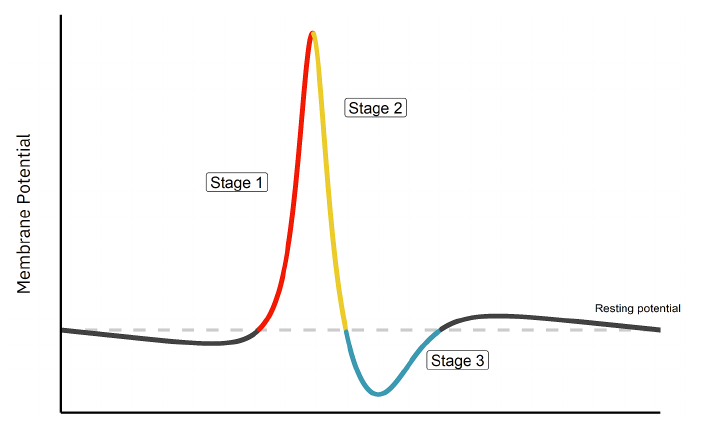
\includegraphics[width=0.5\textwidth]{wave_form.png}
    \end{figure}
\end{frame}
